\documentclass[a4paper]{exam}
\usepackage[margin=1in]{geometry}
\usepackage{amsmath}
\usepackage{geometry}
\usepackage{hyperref}
\usepackage{pythonhighlight}
\usepackage{listings}
\usepackage{xcolor}
\usepackage{graphicx}

\definecolor{codegreen}{rgb}{0,0.6,0}
\definecolor{codegray}{rgb}{0.5,0.5,0.5}
\definecolor{codepurple}{rgb}{0.58,0,0.82}
\definecolor{backcolour}{rgb}{0.95,0.95,0.92}

\lstdefinestyle{mystyle}{
    backgroundcolor=\color{backcolour},   
    commentstyle=\color{codegreen},
    keywordstyle=\color{magenta},
    numberstyle=\tiny\color{codegray},
    stringstyle=\color{codepurple},
    basicstyle=\ttfamily\footnotesize,
    breakatwhitespace=false,         
    breaklines=true,                 
    captionpos=b,                    
    keepspaces=true,                 
    numbers=left,                    
    numbersep=5pt,                  
    showspaces=false,                
    showstringspaces=false,
    showtabs=false,                  
    tabsize=2
}

\lstset{style=mystyle}
\printanswers

\begin{document}
\begin{center}
{\Large \textbf{Spring 2024}}\vspace{1.0em}\\
{\Large \textbf{CS 412 (Algorithms: Design and Analysis)}}\vspace{1.0em}\\
{\Large \textbf{Weekly Challenge 08: Dynamic Programming}}\vspace{1.0em}\\
{\Large Announced: Friday, March 15, 2024.}\\
\vspace{.25em}
{\Large Deadline: Friday, March 29, 2024 (11:59 pm PKT).}\\ 
\vspace{.3em}
{\Large Total marks: 2.}
\vspace{.5em}\\
\end{center}
\textbf{Instructions}: Submit \textbf{individually} your solution as a PDF (\textit{studentID.pdf}) typeset in LaTeX and Zip (\textit{studentID\_WC8\_DP.zip}) for the code. You must submit your solution on Canvas.

\centerline{\rule{.7\textwidth}{1pt}}
\begin{questions}
\question[1]
  We are going to implement the rod cutting algorithm from CLRS 15.1 in a file \texttt{cutrod.py}. We will implement the following three versions of the solution: \textit{top-down recursive}, \textit{top-down memoized}, and \textit{bottom-up}. Your code will be tested by \pyth{pytest} using the file, \texttt{test\_cutrod.py}, given in \texttt{WC8\_DP.zip}. To test your code implementation, open the directory containing \texttt{test\_cutrod.py} and \texttt{cutrod.py} in the terminal, and run the following command:
\begin{lstlisting}[language=bash]
pytest test_cutrod.py
\end{lstlisting}
  \textbf{TASKS}:
  \begin{parts}
  \part Write the top-down recursive version in a function, \pyth{cut_rod}.
  \part Write the top-down memoized version in a function, \pyth{cut_rod_memoized}.
  \part Write the bottom-up version in a function, \pyth{cut_rod_bottom_up}.
  \part All functions take two arguments, \texttt{p} and \texttt{n}, where \texttt{p} is the price array and \texttt{n} is the length of the rod. \texttt{p[i]} is the price of a rod of length \texttt{i}. All prices are positive and increase with length.
  \part Write all functions in the file, \texttt{cutrod.py}.
  \part Ensure that all tests pass by running \pyth{pytest} locally.
  \part Do not include any external packages.  
  \part You may modify the error messages in \texttt{test\_cutrod.py} to convey more information if you wish, but you may not alter any other functionality in it.
  \part Plot the running time of the three versions against \texttt{n} and include them below along with any relevant observations. Your code for plotting should be in \texttt{plot.py}. 
  \end{parts}

  
  \begin{solution}
    The codes are in the ZIP file attached.

    \begin{center}
      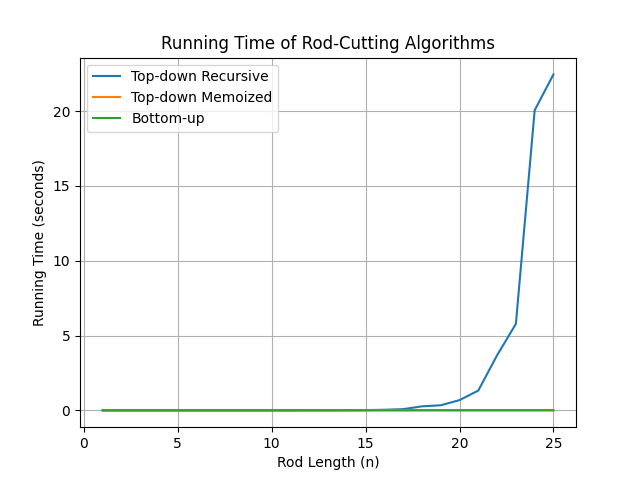
\includegraphics[width=0.8\textwidth]{Figure_1.png}
    \end{center}
    It is important to note that the running time complexities of these algorithms where the Top-down recursive function has exponential time complexity
    The exponential term in the top-down recursive solution makes it significantly slower than the other two for larger values of n. Even though both memoized and bottom-up solutions have a $n^2$ term, the constant factors involved in each algorithm's implementation can affect the observed runtime.
  \end{solution}
\end{questions}
\end{document}

%%% Local Variables:
%%% mode: latex
%%% TeX-master: t
%%% End:
